\documentclass[10pt,a4paper]{article}
\usepackage[T2A]{fontenc}
\usepackage[utf8]{inputenc}
\usepackage[english,russian]{babel}
\usepackage[margin=2cm]{geometry}
\usepackage{amsmath,amssymb}
\usepackage{graphicx,booktabs,array,xcolor}
\usepackage[hidelinks]{hyperref}
\usepackage{caption}
\captionsetup{font=small,labelfont=bf}
\setlength{\parskip}{3pt}
\newcommand{\mg}{\mathrm{MG}}
\newcommand{\good}[1]{\textcolor[HTML]{117733}{#1}}
\newcommand{\bad}[1]{\textcolor[HTML]{BB5566}{#1}}
\graphicspath{{./}{../}}

\title{MG по скалярному логу как дешёвый индикатор упрощения обучения:\\
сводный отчёт по экспериментам}
\author{Проект 202, эксперименты 29 сентября --- 1 октября 2026}
\date{}

\begin{document}
\maketitle

\section*{Итог}

Цель серии --- собрать прикладные примеры, в которых оценка MacKay--Ghahramani (MG),
посчитанная по одному скалярному логу обучения, отмечает момент, когда обучение
\emph{действительно} упростилось, а само упрощение установлено независимо. Проведено
шесть экспериментов на CPU и один на GPU (Colab); все скрипты, сырые логи и таблицы лежат в
\texttt{research\_trajectory\_reference/}.

\begin{table}[h]
\centering\small
\begin{tabular}{@{}p{3.4cm}p{3.6cm}p{4.3cm}p{4.2cm}@{}}
\toprule
Эксперимент & Упрощение и его подтверждение & Что показал MG & Вывод \\
\midrule
1. Пилот: MLP, digits, SGD & спад lr, заморозка; PR траектории весов
  & лог loss: падает при упрощении (AUC 0.99), но MG совпадает с MG суррогата
  & \bad{под SGD MG по loss --- функция спектра} \\
2. MLP, full batch, большой шаг & --- & MG заметно ниже суррогата (0.51--0.66),
  устойчив к сглаживанию лога & в детерминированном режиме у MG есть своя информация \\
3. Edge of stability (E2) & число мод Гессиана на пороге $2/\eta$, Ланцош
  & \bad{антикорреляция} с числом мод ($\rho=-0.83$) & \bad{отрицательный} \\
4. CNN, CIFAR-10, три события (E4) & спад lr, заморозка, прунинг --- по построению
  & лог нормы параметров: $-8\ldots-13\,\%$, контроли $\geq -3\,\%$, AUC 0.98
  & \good{положительный, эффект небольшой} \\
5. То же, события по дозам (E5) & то же + PR ковариации обновлений весов
  & сильные события $-12\ldots-19\,\%$, контроли $0\ldots+13\,\%$; AUC 0.93, для
    сильнейших доз 0.99; простые статистики $\approx 0.5$
  & \good{положительный, подтверждён на новых сидах} \\
6. Онлайн-детектор (E6) & как в 5 & порог с других сидов: пойманы 27/28 сильных событий,
    0/16 ложных тревог; простые статистики --- 31--62\,\% ложных тревог
  & \good{положительный} \\
7. ResNet-18, полный CIFAR-10, с нуля и дообучение (E7, E7b) & как в 5 + PR обновлений по CountSketch
  & норма параметров --- гладкая кривая: ловится только заморозка ($-28\ldots-31\,\%$, 6/6);
    lr и прунинг --- 0/24; проекции и нормы слоёв: тревоги без различия событий и контролей
  & \bad{на большой сети не переносится} \\
\bottomrule
\end{tabular}
\end{table}

\textbf{Главный результат.} В обучении свёрточной сети на CIFAR-10 MG по логу
\emph{нормы параметров} --- величине, которая считается по уже имеющимся весам за
$O(P)$ и не требует ни одного прохода сети, --- падает после явных событий упрощения
(заморозка всего, кроме головы; прунинг; спад learning rate в 10--100 раз) на
$12$--$19\,\%$ в медиане и не падает в контролях без упрощения (обучение без события,
меньший шум градиента, масштаб и сглаживание лога). Простые статистики того же лога
(пересечения тренда, автокорреляция, разброс) события не отделяют (AUC около 0.5).
Результат воспроизвёлся на сидах, которые не участвовали в выборе настроек. Онлайн-детектор с порогом, выбранным на других сидах, поймал 27 из 28 запусков с сильным упрощением и не дал ни одной ложной тревоги в 16 запусках без упрощения; детекторы на простых статистиках ложно срабатывают в 31--62\,\% таких запусков.

\textbf{Главное ограничение: на большой сети результат не переносится.} На ResNet-18
(11 млн параметров, полный CIFAR-10, 42 запуска на GPU) лог нормы параметров
превращается в гладкую монотонную кривую: колебания усредняются по 11 млн
координат. MG на нём стоит на постоянном значении гладкого транзиента и ловит только
заморозку всей сети, кроме головы ($-28\ldots-31\,\%$, 6 из 6, без ложных тревог).
Спад learning rate и прунинг он не видит (0 из 24). Наблюдатели с сохранёнными
колебаниями --- случайные проекции параметров, нормы отдельных слоёв --- шумовые:
MG на них падает при сглаживании лога и растёт при уменьшении шума, а детектор
срабатывает одинаково часто на событиях (63\,\%) и без них (71\,\%).

\textbf{Прочие границы.} Эффект составляет десятки процентов, а не кратное изменение; слабые
события (lr$/3$, заморозка двух первых слоёв) MG не видит; как размерность число
читать нельзя (отношение идентифицируемости $\approx 1.5$). Под SGD MG по логу loss
не даёт ничего сверх спектра, а на edge of stability меняется в направлении,
обратном числу колеблющихся мод. Сильный положительный пример с кратным эффектом
получен пока только в детерминированной системе (FORCE-эксперимент, папка
\texttt{best\_exp}, снижение на 68--80\,\%).

\section{Вопрос и методика}

\paragraph{Тезис статьи, который проверяется.} Теоретически MG по
delay-реконструкции скаляра меряет число активных компонент детерминированного
возвратного режима; на синтетике так и происходит. Для реального обучения нужен
более слабый, но полезный тезис: MG --- дешёвый индикатор упрощения динамики,
который прикручивается к любому уже записанному логу.

\paragraph{Почему предыдущие попытки (neural collapse, LLM) не подтвердили тезис.}
MG сравнивали с величинами другого типа: геометрией признаков (NC1/NC2),
кривизной Гессиана, PR активаций. MG описывает движение траектории
оптимизации, поэтому эталон должен описывать то же движение: число направлений,
по которым меняются веса, или число колеблющихся мод.

\paragraph{Общая схема.} В середине обучения происходит одно событие. По окнам лога
считается MG, берётся медиана по окнам до события и после, и сравнивается их
отношение. В каждом эксперименте есть три контроля: масштаб лога (MG обязан не
измениться), сглаживание лога скользящим средним (траектория та же, наблюдатель
другой) и увеличенный батч (меньше шума при тех же движущихся параметрах). Кроме
того, для каждого окна считается MG трёх IAAFT-суррогатов --- рядов с тем же
спектром, но без нелинейной структуры. Отношение MG$/$MG\textsubscript{сурр}$\approx 1$
означает, что вся информация лога в спектре.

\paragraph{Оценщик.} Реализация проекта без изменений ядра (pooled MG, исключение
Тейлера на размах вектора задержек). Эксперименты 1--4: $E=10$, $\tau=1$, $k=10$;
эксперимент 5: конфигурация статьи $E=20$, $\tau=1$, $k=20$, окно 1\,000 шагов.

\section{Эксперимент 1. Пилот: MLP на digits, SGD}

MLP $64\!-\!64\!-\!64\!-\!10$ (9\,290 параметров), sklearn digits, SGD, 6\,000 шагов,
событие на шаге 3\,000, 5 сидов. Эталон --- detrended PR траектории всех весов
в окне 500 шагов.

\begin{figure}[h]
\centering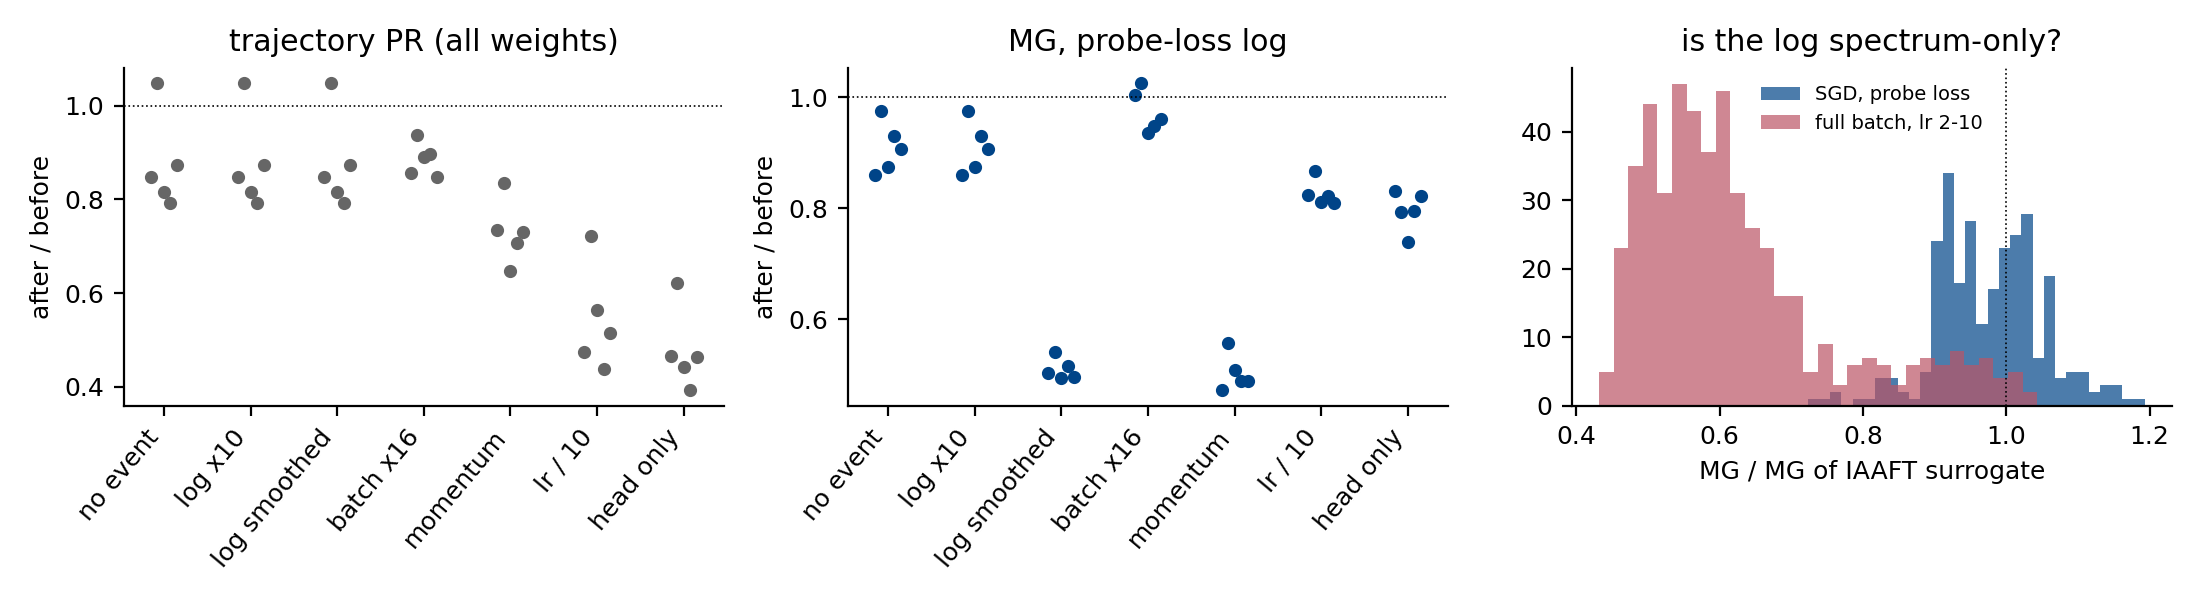
\includegraphics[width=\textwidth]{report/pilot_summary.png}
\caption{Пилот. Слева и в центре --- отношение после/до для эталона и для MG
лога loss на фиксированном probe. Справа --- распределение MG$/$MG суррогата по
окнам: под SGD оно сосредоточено у 1, в полнобатчевом режиме с большим шагом ---
заметно ниже 1.}
\end{figure}

\begin{table}[h]\centering\small
\begin{tabular}{lcccc}\toprule
событие & PR траектории & MG, probe loss & пересечения тренда & MG$/$суррогат\\\midrule
нет & 0.85 & 0.91 & 0.63 & 1.04\\
батч $\times16$ & 0.89 & 0.96 & 0.73 & 1.03\\
lr $/10$ & \textbf{0.51} & \textbf{0.82} & 0.32 & 1.06\\
учится только голова & \textbf{0.46} & \textbf{0.80} & 0.27 & 1.06\\
лог сглажен (траектория та же) & 0.85 & \bad{0.50} & 0.18 & 1.03\\
\bottomrule\end{tabular}
\caption{Отношение после/до, медиана по 5 сидам.}\end{table}

MG разделяет упростившиеся и контрольные запуски (AUC 0.99; корреляция отношений с
эталоном $\rho=0.85$). Однако отношение к суррогату равно 1 (медиана 0.98,
межквартильный размах 0.93--1.03): под SGD лог loss --- окрашенный шум, и MG на нём
определяется одним спектром, как предсказывают Osborne и Provenzale (1989). Поэтому
пересечения тренда делают то же самое, а сглаживание лога даёт ложную тревогу.
Адаптивный лаг снимает ложную тревогу, но тогда знак отклика на заморозку и спад
lr меняется на противоположный (1.60 и 1.45).

\section{Эксперимент 2. Полный батч, большой шаг}

Та же сеть, полнобатчевый спуск с шагом $\eta\in\{0.5,2,5,10\}$. При $\eta\geq 2$ loss
колеблется сам, без шума выборки. MG в этом режиме в 1.5--2 раза ниже суррогатного
(отношение 0.66, 0.58, 0.51): в логе есть детерминированная нелинейная структура.
После сглаживания лога MG меняется слабо (0.87--1.15), а MG суррогата и пересечения
тренда падают (0.62--0.80 и 0.27--0.56). Это режим, где теория применима и у MG есть
информация, недоступная спектральным статистикам.

\section{Эксперимент 3 (E2). Edge of stability: число колеблющихся мод}

\paragraph{Постановка.} MLP на digits, MSE, полнобатчевый спуск,
$\eta\in\{0.05,\dots,0.4\}$, 5 сидов, 8\,000 шагов, плюс переключения $\eta$ вниз на
середине. На edge of stability несколько собственных значений Гессиана держатся на
пороге $2/\eta$; их число растёт с $\eta$. Эталоны: число таких мод (Ланцош по
произведениям Гессиана на вектор каждые 250 шагов) и PR траектории весов.

\begin{figure}[h]
\centering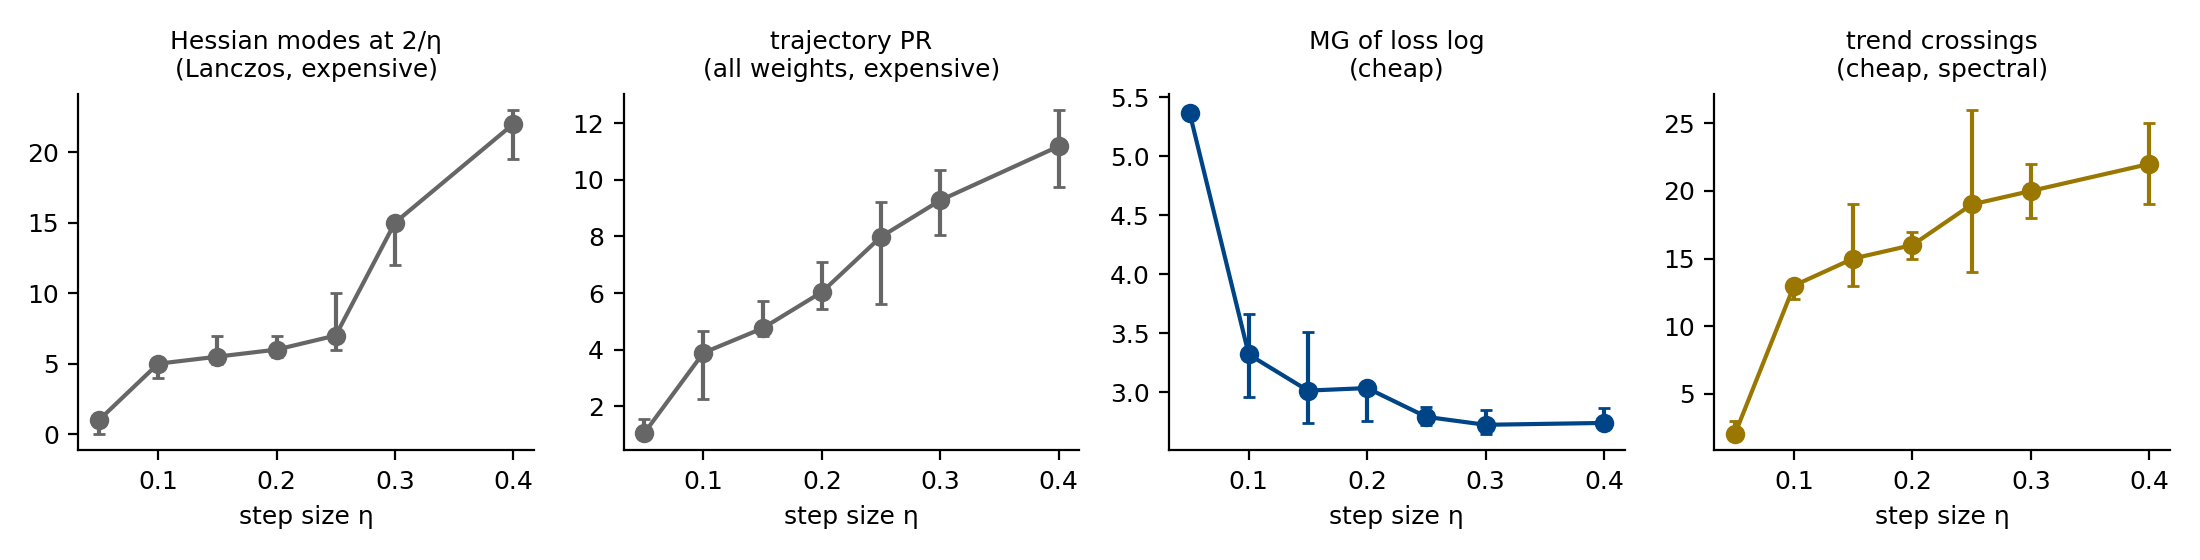
\includegraphics[width=\textwidth]{results_eos/figures/sweep_levels.png}
\caption{Уровни по шагу $\eta$: два дорогих эталона растут, MG падает.}
\end{figure}

\paragraph{Результат (отрицательный).} Число мод растёт от 1 до 22, PR траектории ---
от 1.05 до 11.2, а MG падает от 5.4 до 2.7. Ранговая корреляция MG с числом мод
$\rho=-0.83$ по запускам и $-0.73$ по окнам; пересечения тренда коррелируют
правильно ($+0.90$). При уменьшении шага моды уходят с порога и PR траектории падает
в 3--4 раза, а MG почти удваивается (${\times}1.8$): лог становится гладким
транзиентом, на котором MG выходит на постоянное значение конфигурации. Отношение
идентифицируемости во всех окнах 1.3--1.7, то есть диагностики статьи
предупреждают, что уровень не является размерностью. Убрать из лога колебание с
периодом 2 перед вложением пробовали всеми способами (все варианты перечислены
в \texttt{REPORT\_E2\_ru.md}); знак не исправляется.

\begin{figure}[h]
\centering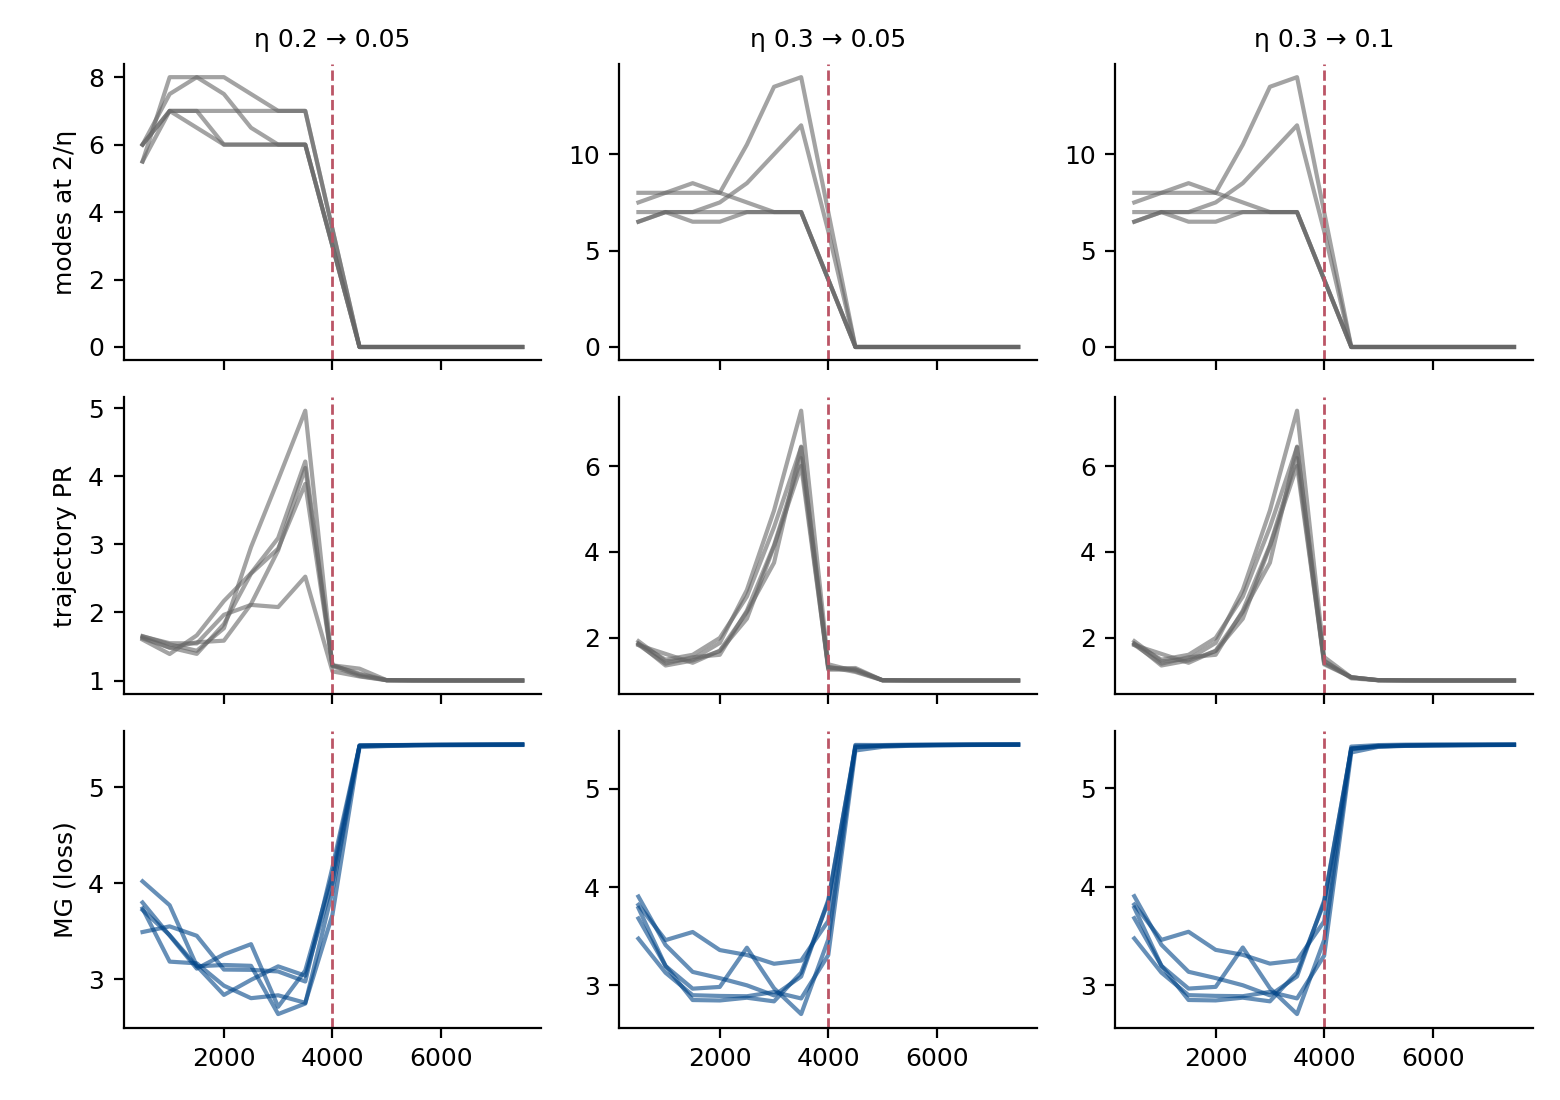
\includegraphics[width=0.78\textwidth]{results_eos/figures/switch.png}
\caption{Переключение шага на середине (пунктир): моды уходят с порога, PR
траектории падает, MG растёт.}
\end{figure}

\section{Эксперимент 4 (E4). CNN на CIFAR-10: три практических события}

\paragraph{Постановка.} CIFAR-10, 10\,000 обучающих изображений (по 1\,000 на
класс). CNN из трёх свёрток и линейной головы, 14\,666 параметров. SGD с momentum
0.9, weight decay $5\cdot10^{-4}$, lr 0.02, батч 64, 8\,000 шагов, событие на шаге
4\,000, 4 сида. Тестовая точность 0.61--0.64 во всех рукавах.

События, для которых упрощение известно по построению:
\begin{itemize}\setlength\itemsep{0pt}
\item lr$/10$ --- шаг и шум в 10 раз меньше;
\item обучается только голова --- 330 из 14\,666 параметров;
\item прунинг 80\,\% весов по модулю.
\end{itemize}
Логи: loss мини-батча, loss на фиксированных 100 изображениях, норма градиента,
норма параметров.

\paragraph{Эталон PR траектории под SGD непригоден.} PR траектории всех весов почти
не меняется ни при одном событии, в том числе при заморозке (0.92). Моделирование
показало причину: detrended PR чистого случайного блуждания на 500 шагах равен
$\approx 5$ при любой размерности пространства (5.08 при $P=330$, 5.04 при
$P=14\,666$). Под SGD эта величина описывает форму блуждания, а не число движущихся
направлений. В эксперименте 5 эталон заменён на PR ковариации \emph{обновлений}
весов.

\begin{figure}[h]
\centering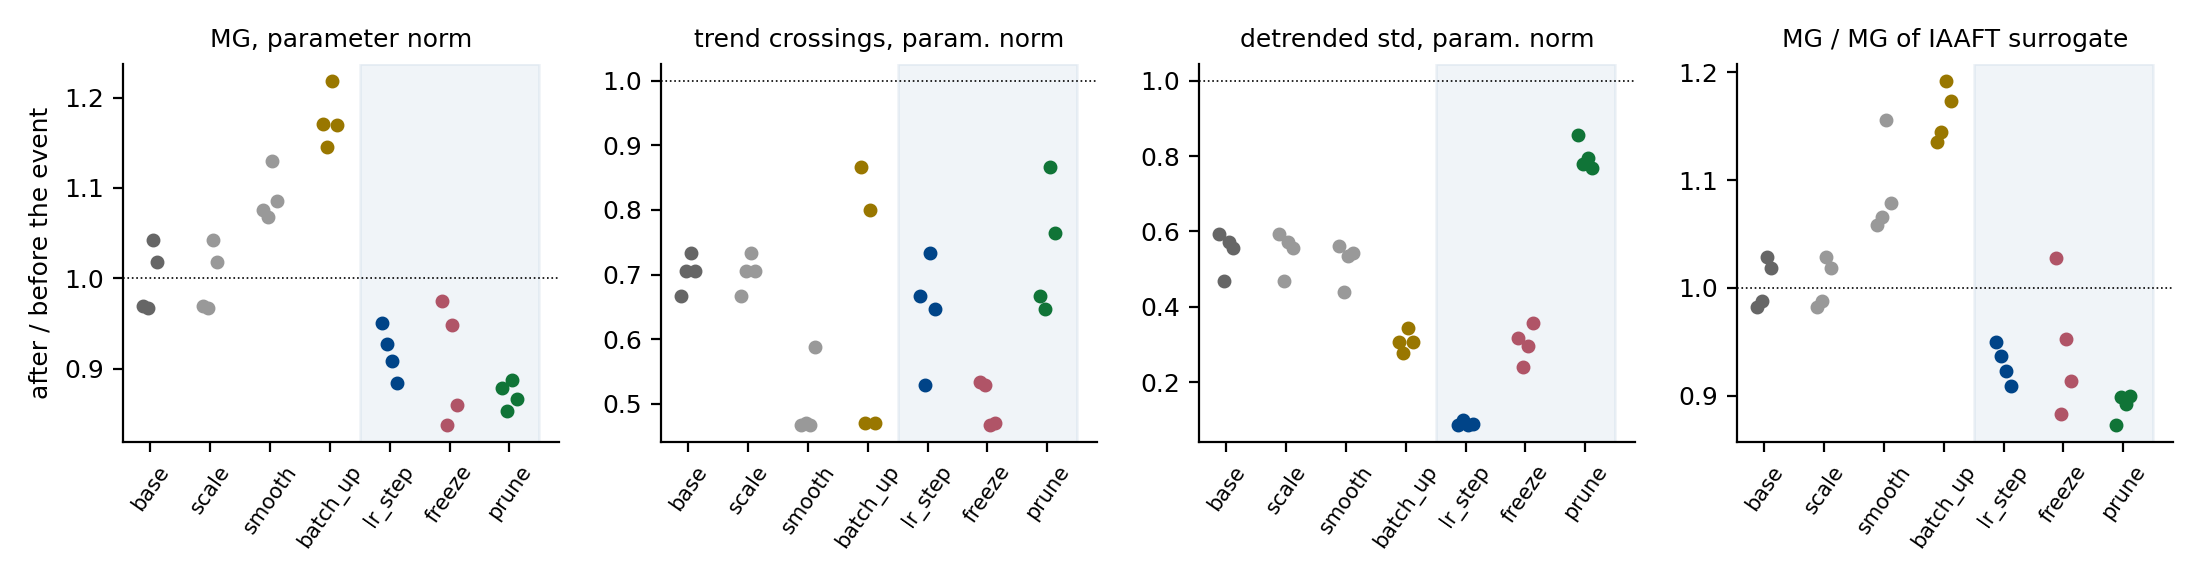
\includegraphics[width=\textwidth]{results_cifar/figures/paramnorm_ratios.png}
\caption{Лог нормы параметров, отношение после/до по запускам. Затенено ---
события упрощения.}
\end{figure}

\paragraph{Результат.} Норма параметров:
\begin{itemize}\setlength\itemsep{0pt}
\item MG после события: lr$/10$ \textbf{$-8\,\%$}, заморозка \textbf{$-10\,\%$},
  прунинг \textbf{$-13\,\%$};
\item контроли: без события $-1\,\%$, масштаб $-1\,\%$, сглаживание $+8\,\%$,
  батч$\times4$ $+17\,\%$;
\item все 12 событийных значений не выше $-3\,\%$, все контрольные не ниже $-3\,\%$;
  AUC 0.98;
\item пересечения тренда, автокорреляция и разброс того же лога: AUC 0.64, 0.41,
  0.58;
\item MG$/$суррогат 0.80, и сдвиг MG не спектральный.
\end{itemize}

Логи loss: MG по probe loss видит события, но только через спектр (отношение к
суррогату 1.00, те же AUC у простых статистик, ложная тревога ${\times}0.66$ при
сглаживании). MG по loss мини-батча не реагирует ни на что: его колебания задаёт
выборка батча.

\section{Эксперимент 5 (E5). События по дозам, подтверждение на новых сидах}

\paragraph{Что изменено и почему.} Две настройки выбраны по логам эксперимента 4
(сиды 0--3) и затем зафиксированы в протоколе:
\begin{itemize}\setlength\itemsep{0pt}
\item наблюдатель --- норма параметров;
\item конфигурация статьи $E=20$, $\tau=1$, $k=20$, окно 1\,000.
\end{itemize}
Сам эксперимент проведён на новых сидах 10--13, поэтому выбор настроек не влияет
на его числа. Упрощения сделаны явнее и по дозам, а после события отводится больше
шагов: 10\,000 шагов, событие на 4\,000, окна после события начинаются в
[5\,000, 9\,000].

Независимое подтверждение измеряется:
\begin{itemize}\setlength\itemsep{0pt}
\item доля параметров, которые двигаются;
\item PR ковариации обновлений весов --- в отличие от PR траектории, у неё нет
  артефакта случайного блуждания;
\item средний размер обновления.
\end{itemize}

\begin{table}[h]\centering\footnotesize
\begin{tabular}{lcccccc}\toprule
событие & MG до & MG после & изменение & разброс по сидам & PR обновлений & двигается\\\midrule
без события & 4.31 & 4.32 & $+0.4\,\%$ & $-8.7\ldots+3.3$ & $+40\,\%$ & 100\,\%\\
батч $\times4$ (меньше шума) & 4.31 & 4.85 & $+12.8\,\%$ & $+8.3\ldots+13.9$ & $-7\,\%$ & 100\,\%\\
лог $\times10$ & 4.31 & 4.32 & $+0.4\,\%$ & как без события & --- & ---\\
лог сглажен & 4.31 & 4.44 & $+3.4\,\%$ & $-5.1\ldots+4.2$ & --- & ---\\\midrule
lr $/3$ & 4.31 & 4.35 & $+0.9\,\%$ & $-6.8\ldots+4.2$ & $-5\,\%$ & 100\,\%\\
lr $/10$ & 4.31 & 3.95 & $\mathbf{-8.3\,\%}$ & $-12.1\ldots-2.3$ & $-22\,\%$ & 100\,\%\\
lr $/100$ & 4.31 & 3.85 & $\mathbf{-11.5\,\%}$ & $-14.4\ldots-7.3$ & $-21\,\%$ & 100\,\%\\\midrule
заморожены conv1--2 & 4.31 & 4.27 & $-1.8\,\%$ & $-3.9\ldots+2.2$ & $-14\,\%$ & 65\,\%\\
учится только голова & 4.31 & 3.51 & $\mathbf{-18.5\,\%}$ & $-24.1\ldots-11.2$ & $-43\,\%$ & 2.2\,\%\\
учится только bias головы & 4.31 & 3.58 & $\mathbf{-16.7\,\%}$ & $-23.7\ldots-15.0$ & $-68\,\%$ & 0.07\,\%\\\midrule
прунинг 50\,\% & 4.31 & 3.80 & $\mathbf{-12.7\,\%}$ & $-14.5\ldots-3.9$ & $+15\,\%$ & 50\,\%\\
прунинг 80\,\% & 4.31 & 3.59 & $\mathbf{-17.5\,\%}$ & $-20.7\ldots-12.3$ & $-10\,\%$ & 20\,\%\\
прунинг 95\,\% & 4.31 & 3.79 & $\mathbf{-11.5\,\%}$ & $-16.1\ldots-9.5$ & $-45\,\%$ & 6\,\%\\
\bottomrule\end{tabular}
\caption{MG лога нормы параметров до и после события: медиана по 4 сидам и
диапазон по сидам. PR обновлений и доля движущихся параметров --- независимое
дорогое подтверждение.}\end{table}

\begin{figure}[h]
\centering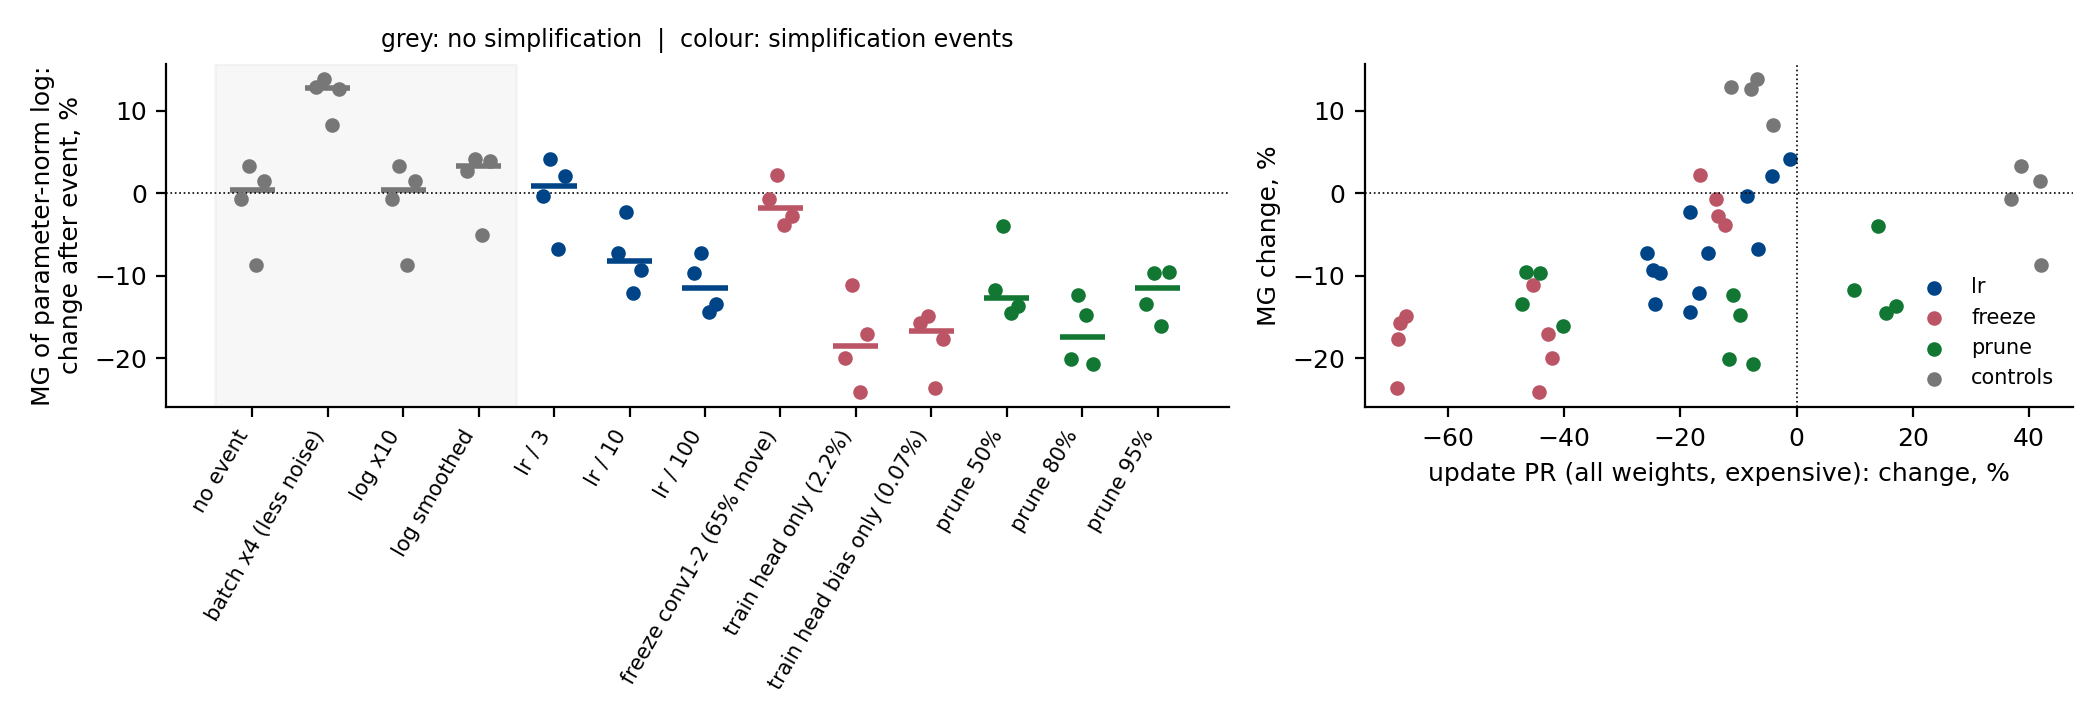
\includegraphics[width=\textwidth]{results_graded/figures/mg_change.png}
\caption{Слева --- изменение MG после события для каждого запуска (черта ---
медиана); серый фон --- контроли без упрощения. Справа --- изменение MG против
изменения PR обновлений всех весов.}
\end{figure}

\paragraph{Проверка заранее записанных предсказаний.}
\begin{itemize}\setlength\itemsep{1pt}
\item \textbf{P1: медиана каждого события ниже медианы каждого контроля ---
  \bad{не выполнено}.} Самые слабые дозы (lr$/3$: $+0.9\,\%$; заморозка conv1--2:
  $-1.8\,\%$) неотличимы от контроля. По эталону они и меняют движение слабее
  всего: PR обновлений $-5\,\%$ и $-14\,\%$.
\item \textbf{P2: сильнейшая доза ниже каждого контрольного запуска} ---
  \good{выполнено} для заморозки и прунинга; для lr \bad{не выполнено}: один сид
  lr$/100$ ($-7.3\,\%$) выше одного сида без события ($-8.7\,\%$).
\item \textbf{P3: монотонность по дозе} --- \good{да} для lr ($\rho=-0.83$) и для
  заморозки ($-0.68$); для прунинга \bad{нет} ($\rho=-0.03$: 80\,\% сильнее, чем
  95\,\%).
\item \textbf{P4: контроли не дают ложной тревоги} --- \good{выполнено}: масштаб
  $0\,\%$, сглаживание $+3\,\%$, меньший шум $+13\,\%$.
\end{itemize}

\paragraph{Сравнение с простыми статистиками того же лога.} AUC «событие против
контролей без упрощения»:

\begin{center}\small
\begin{tabular}{lccccc}\toprule
& MG & MG сурр. & пересеч. тренда & автокорр. & разброс\\\midrule
все события & \textbf{0.93} & 0.68 & 0.56 & 0.48 & 0.57\\
сильнейшие дозы, все контроли & \textbf{0.99} & --- & 0.52 & 0.48 & 0.67\\
\bottomrule\end{tabular}
\end{center}

MG по loss мини-батча: AUC 0.19, то есть знак обратный и эффект слабый. Корреляция
изменения MG с изменением PR обновлений по всем запускам $\rho=0.59$. Отношение
MG$/$суррогат 0.78: изменение MG не сводится к спектру.

\begin{figure}[h]
\centering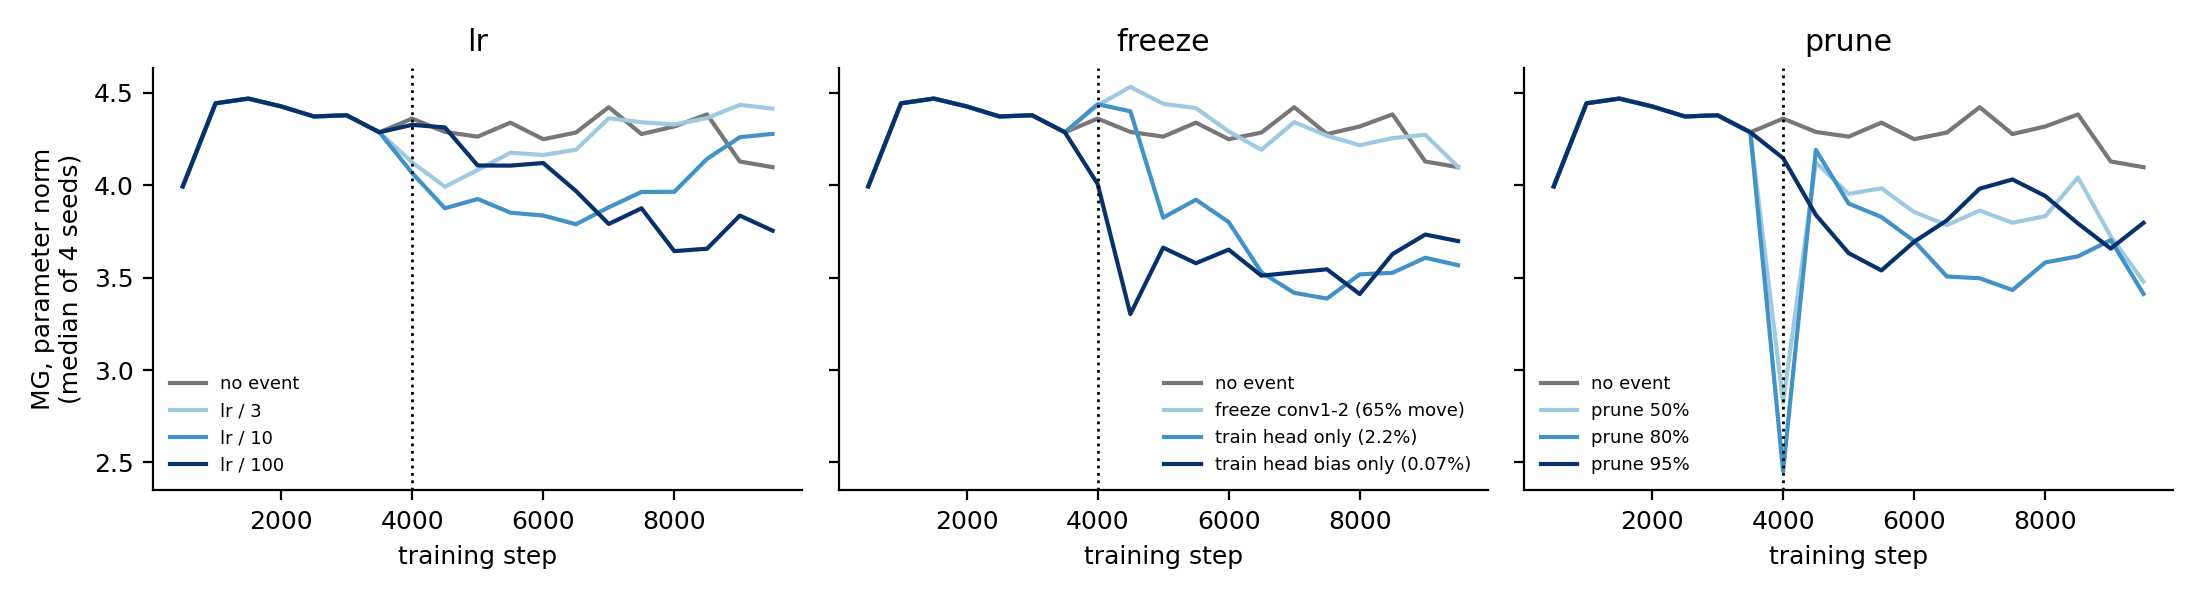
\includegraphics[width=\textwidth]{results_graded/figures/time_courses.png}
\caption{MG во времени, медиана по 4 сидам. При прунинге окно, накрывающее сам шаг
4\,000, падает до $\approx 2.4$: норма там скачком меняется. Такие окна в сравнение
не входят --- «после» начинается с шага 5\,000.}
\end{figure}

\section{Эксперимент 6 (E6). Онлайн-детектор упрощения}

\paragraph{Зачем.} Сравнение медиан «до/после» предполагает, что момент события
известен. Практику нужен монитор, который сам поднимает тревогу, и важно знать,
насколько поздно он это делает и как часто срабатывает без причины. Детектор
построен на уже записанных логах нормы параметров, без переобучения; протокол ---
в docstring \texttt{detector.py}.

\paragraph{Правило.} Для окна $k$ считается относительное падение
\[
D_k=\frac{\operatorname{med}(\mg_{k-M+1..k})}{\operatorname{med}(\mg_{k-M-B+1..k-M})}-1,
\]
то есть медиана последних $M$ окон против медианы $B$ окон перед ними. Тревога
поднимается при первом $D_k<-\delta$. Параметры $(M,B,\delta)$ подбираются \emph{только
на сидах эксперимента~4} (0--3) так, чтобы не было ни одной тревоги в запусках без
события. Проверка --- на сидах эксперимента~5 (10--13) со всеми его рукавами и
контролями. Выбрано $M=2$, $B=3$, $\delta=8.8\,\%$. Тем же способом откалиброваны
детекторы на простых статистиках того же лога.

\begin{center}\small
\begin{tabular}{lccccc}\toprule
статистика в детекторе & \multicolumn{2}{c}{доля пойманных событий} & ложные тревоги & медианная\\
& сильные (28) & слабые (8) & без упрощения (16) & задержка\\\midrule
\textbf{MG} & \good{\textbf{0.96}} & 0.25 & \good{\textbf{0.00}} & 1\,000 шагов\\
разброс лога (detrended std) & 1.00 & 0.75 & \bad{0.62} & 500 шагов\\
пересечения тренда & 0.54 & 0.12 & \bad{0.31} & 1\,000 шагов\\
автокорреляция & 0.00 & 0.00 & 0.00 & ---\\
\bottomrule\end{tabular}
\end{center}

MG по рукавам:
\begin{itemize}\setlength\itemsep{0pt}
\item прунинг 50/80/95\,\%, обучение одной головы и одного bias --- пойманы во всех
  4 сидах;
\item lr$/100$ --- 4 из 4; lr$/10$ --- 3 из 4;
\item слабые события: lr$/3$ --- 2 из 4, заморозка conv1--2 --- 0 из 4;
\item без события, меньший шум, масштаб, сглаживание --- ни одной тревоги.
\end{itemize}
Детектор по разбросу лога тоже ловит все события, но ложно срабатывает при
масштабировании лога (4 из 4), обычном обучении и меньшем шуме (по 2 из 4).

\begin{figure}[h]
\centering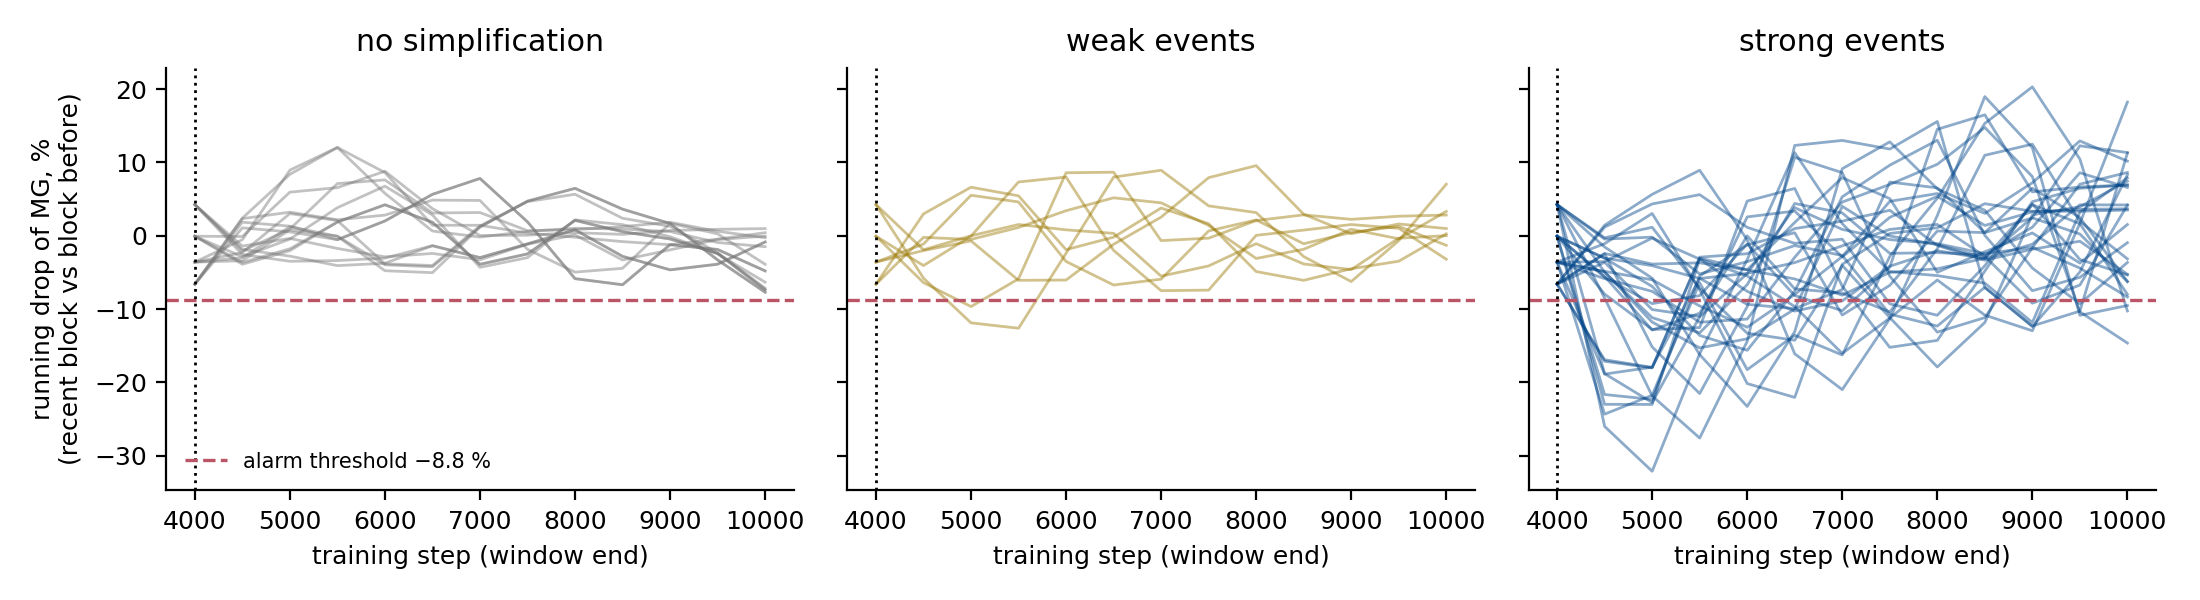
\includegraphics[width=\textwidth]{results_detector/detector_traces.png}
\caption{Статистика детектора $D_k$ по всем тестовым запускам; пунктир --- порог
$-8.8\,\%$, выбранный на других сидах.}
\end{figure}

\paragraph{Ограничения.} Статистике нужны 5 окон истории, поэтому первое значение
появляется на шаге 4\,000, то есть в момент события. Ложные тревоги проверялись на
6\,000 шагах после этого в 16 запусках без упрощения; участок до события
детектором не покрыт. Задержка 1\,000 шагов --- это одна длина окна. При прунинге
часть срабатываний вызвана скачком нормы в момент обнуления весов.

\section{Эксперимент 7 (E7, E7b). ResNet-18 на полном CIFAR-10}

\paragraph{Постановка.} Протокол с предсказаниями записан до запуска
(\texttt{colab\_resnet/PROTOCOL.md}). ResNet-18 обучалась на полном CIFAR-10 в двух
сценариях: с нуля (CIFAR-вариант, $32\times32$) и дообучение ImageNet-предобученной
модели ($64\times64$). SGD с momentum, lr 0.02, батч 128, AMP, 10\,000 шагов, событие
на шаге 4\,000, сиды 20--22. Рукава: без события, батч$\times4$, lr$/10$, lr$/100$,
обучение одной головы, прунинг 80\,\% и 95\,\%; плюс контроли масштаба и сглаживания
лога. Тестовая точность 0.80--0.83 с нуля и 0.86--0.91 при дообучении. Всё
заморожено из экспериментов 5--6: конфигурация MG, окна, правило детектора. Эталон ---
PR ковариации обновлений всех весов через CountSketch до 1\,024 координат.

\paragraph{E7: лог нормы параметров.}
\begin{center}\small
\begin{tabular}{lccc}\toprule
событие & изменение MG, с нуля & при дообучении & детектор поймал\\\midrule
без события / масштаб / сглаживание & $-1.6$ / $-1.6$ / $-1.4\,\%$ & $-1.0$ / $-1.0$ / $-0.9\,\%$ & ложных тревог 0/24\\
батч $\times4$ & $+1.8\,\%$ & $+3.5\,\%$ & ---\\
\textbf{обучается только голова} & $\mathbf{-27.6\,\%}$ & $\mathbf{-30.8\,\%}$ & \good{6/6}\\
lr $/10$ / lr $/100$ & $+2.5$ / $+2.4\,\%$ & $+4.2$ / $+4.0\,\%$ & \bad{0/12}\\
прунинг 80\,\% / 95\,\% & $+1.8$ / $-1.8\,\%$ & $-1.0$ / $-0.5\,\%$ & \bad{0/12}\\
\bottomrule\end{tabular}
\end{center}
PR обновлений при этом падает во всех событиях: при обучении одной головы на
91\,\% с нуля и на 85\,\% при дообучении, при lr$/10$ на 35\,\% и 66\,\%, при
прунинге 80\,\% на 41\,\% с нуля. Предсказания P1 и P2 для спада lr и прунинга
\bad{не выполнены}.

\paragraph{Причина --- наблюдатель.} В каждом окне до события у лога нормы 2
пересечения тренда, а разброс после удаления тренда $\approx 0$: норма по 11 млн
координат --- гладкая монотонная кривая. MG на ней равен значению, которое
конфигурация даёт гладкому транзиенту ($\approx 5.0$ во всех рукавах), и реагирует
только на изменение формы самой кривой, как при заморозке. Это тот же артефакт
транзиента, что в эксперименте 3 и в §6.1 статьи; диагностика (2 пересечения тренда)
его помечает. У малой CNN из экспериментов 4--6 колебания нормы ещё сохранялись.

\paragraph{E7b: наблюдатели с колебаниями.} Протокол записан до анализа
(\texttt{e7b\_analyse.py}). Из уже сохранённых логов, без переобучения, извлечены:
\begin{itemize}\setlength\itemsep{0pt}
\item 16 фиксированных случайных проекций $\theta_t-\theta_0$ --- накопленные суммы
  координат CountSketch обновлений; это наблюдатель «fixed parameter projection»,
  самый точный в §5.2 статьи;
\item нормы слоёв.
\end{itemize}
Основной наблюдатель --- первая проекция, выбранная до просмотра данных.
\begin{center}\small
\begin{tabular}{llcc}\toprule
сценарий & наблюдатель & пойманы сильные события & ложные тревоги\\\midrule
с нуля & проекция 0 & 5/15 & \bad{8/12}\\
дообучение & проекция 0 & 12/15 & \bad{8/12}\\
оба & все 16 проекций & 302/480 (63\,\%) & \bad{271/384 (71\,\%)}\\
оба & медиана MG по 16 проекциям & 0/30 & 6/24\\
с нуля / дообучение & норма \texttt{fc} & 5/15 / 9/15 & \bad{9/12 / 8/12}\\
\bottomrule\end{tabular}
\end{center}
На проекциях MG падает при сглаживании лога на $7$--$18\,\%$, а при меньшем шуме
растёт на $18$--$42\,\%$ в 29 из 32 пар «проекция $	imes$ сценарий». Это тот же спектральный режим, что под SGD в эксперименте~1:
колебания проекции задаёт шум градиента, и MG отражает спектр, а не число
направлений. Детектор на проекциях срабатывает одинаково часто с событием и без него.

\paragraph{Вывод.} Результат экспериментов 4--6 на ResNet-18 не переносится. Два типа
бесплатных скалярных логов большой сети дают два известных режима отказа: норма
всей сети слишком гладкая (транзиент), проекции и нормы слоёв слишком шумовые
(спектр). Надёжно ловится только грубое изменение самой кривой, как заморозка
всей сети, кроме головы.

\section{Стоимость}

\begin{center}\small
\begin{tabular}{p{6.2cm}p{9.8cm}}\toprule
что считается & цена\\\midrule
MG одного окна лога (500--1\,000 точек) & 5--10 мс\\
лог нормы параметров & $O(P)$ на шаг, без прохода сети; 31--39 КБ на запуск\\
PR траектории или обновлений, одно окно & 180--300 мс; нужно хранить все веса: 450--560 МБ на запуск\\
Ланцош по Гессиану (эксперимент 3) & $\approx 100$ мс и $\approx 60$ HVP на чекпойнт\\
loss на фиксированном probe & один дополнительный проход сети на шаг ($+75\,\%$ ко времени обучения малой сети)\\
\bottomrule\end{tabular}
\end{center}

\section{Выводы для статьи}

\begin{enumerate}\setlength\itemsep{2pt}
\item \textbf{Что можно утверждать.} На малой сети MG по бесплатному логу нормы параметров
  воспроизводимо отмечает явные события упрощения обучения CNN: заморозку,
  прунинг, сильный спад learning rate. Эффект $-12\ldots-19\,\%$, контроли
  $0\ldots+13\,\%$, результат воспроизведён на новых сидах, а простые статистики
  того же лога этого не делают. Это прикладной пример в духе тезиса «дешёвый
  анализатор упрощения».
\item \textbf{Как формулировать.} Как относительный сигнал «до/после»: абсолютное
  значение размерностью не является (отношение идентифицируемости $\approx 1.5$).
  Слабые упрощения метод не различает.
\item \textbf{Какой лог брать.} Имеет значение: loss мини-батча бесполезен; MG по
  probe loss --- спектральная сводка с ложной тревогой при сглаживании; норма
  параметров даёт нелинейную информацию. В grokking-разделе статьи используется
  тот же лог.
\item \textbf{Чего утверждать нельзя.} Что MG считает число колеблющихся мод в
  реальном обучении (эксперимент 3 даёт обратный знак) и что под SGD уровень MG
  по loss --- размерность.
\item \textbf{Эталон.} Для SGD-обучения оконный PR траектории весов эталоном
  числа направлений не является (артефакт случайного блуждания); это стоит учесть
  при описании §7.2 статьи.
\item \textbf{Масштаб.} На ResNet-18 этот пример не переносится (эксперимент 7);
  в статье его надо подавать как малый пример с явно указанной границей, а не
  как общий инструмент мониторинга SGD-обучения.
\end{enumerate}

\paragraph{Что дальше.}
\begin{itemize}\setlength\itemsep{1pt}
\item Сеттинг «SGD-обучение CNN» считать закрытым: на большой сети бесплатные логи
  либо гладкие, либо шумовые, и оба режима отказа объяснены.
\item Перейти к grokking --- там падение MG по норме параметров уже совпало с
  упрощением траектории и прошло суррогатный тест; расширить на сиды и задачи, эталон
  --- PR обновлений вместо PR траектории.
\item Нормы отдельных слоёв: локализовать, \emph{какой} слой упростился.
\item Для кратного эффекта --- события, переводящие обучение в детерминированный
  режим, как в FORCE-эксперименте (\texttt{best\_exp}).
\end{itemize}

\section*{Воспроизведение}
\small
Все команды выполняются из \texttt{2026-Project-202/research\_trajectory\_reference}:
\begin{itemize}\setlength\itemsep{0pt}
\item эксперименты 1--2: \texttt{pilot.py}, \texttt{reanalyse.py},
  \texttt{fullbatch.py}; результаты в \texttt{results/};
\item эксперимент 3: \texttt{eos.py}, \texttt{eos\_analyse.py},
  \texttt{eos\_posthoc.py}; результаты в \texttt{results\_eos/};
\item эксперимент 4: \texttt{cifar\_events.py}, \texttt{cifar\_analyse.py},
  \texttt{cifar\_paramnorm.py}; результаты в \texttt{results\_cifar/};
\item эксперимент 6: \texttt{detector.py}; результаты в \texttt{results\_detector/};
\item эксперимент 7: \texttt{colab\_resnet/} (Colab), \texttt{e7b\_analyse.py};
  результаты в \texttt{results\_resnet/};
\item эксперимент 5: \texttt{explore\_observer.py} (выбор настроек на старых
  сидах), \newline\texttt{cifar\_graded.py} (протокол в docstring),
  \texttt{graded\_analyse.py}; результаты в \texttt{results\_graded/}.
\end{itemize}
Подробные отчёты по экспериментам 3 и 4: \texttt{REPORT\_E2\_ru.md},
\texttt{REPORT\_E4\_ru.md}. CPU Intel i5-12500H, PyTorch 2.10 (CPU), без GPU.

\end{document}
